\subsubsection{Modelado en openEHR}

El enfoque de openEHR para el modelado es multinivel. Los modelos son desarrollados y mantenidos por expertos de dominio en su propio nivel \cite{openEHRArchitecture}.

El primer nivel se basa en el modelo de referencia. El modelo de referencia corresponde al modelo de información estable, por ejemplo, tipos de datos o estructuras de datos. Todos los datos EHR en cualquier sistema openEHR obedecen el modelo de referencia. Solo este primer nivel es implementado en software \cite{openEHRArchitecture}.

El siguiente nivel consiste en los arquetipos. Los arquetipos corresponden a los contenidos del dominio, por ejemplo, medidas de la presión sanguínea o resultado de la prueba para diabetes. Estos arquetipos son modelados por profesionales clínicos o expertos en informática de la salud sin ningún conocimiento tecnológico de los sistemas finales. Los arquetipos son almacenados en sus propios repositorios.

Las plantillas constituyen el siguiente nivel. Estas plantillas especifican grupos de arquetipos que se usan para un propósito particular, y a menudo corresponden a formularios de pantalla \cite{openEHRArchitecture}.

En el último nivel se encuentran los artefactos generados a partir de las plantillas \cite{openEHR}. Los artefactos, mostrados en la Figura \ref{fig:openeEHR_ecosystem}, no se modelan manualmente. Esto significa que un modelo para resultado de microbiología solo necesita hacerse una vez para habilitar los informes, formularios de interfaz de usuario, documentos y otros formatos de mensaje que se generarán.

\begin{figure}[h]
  \centering
  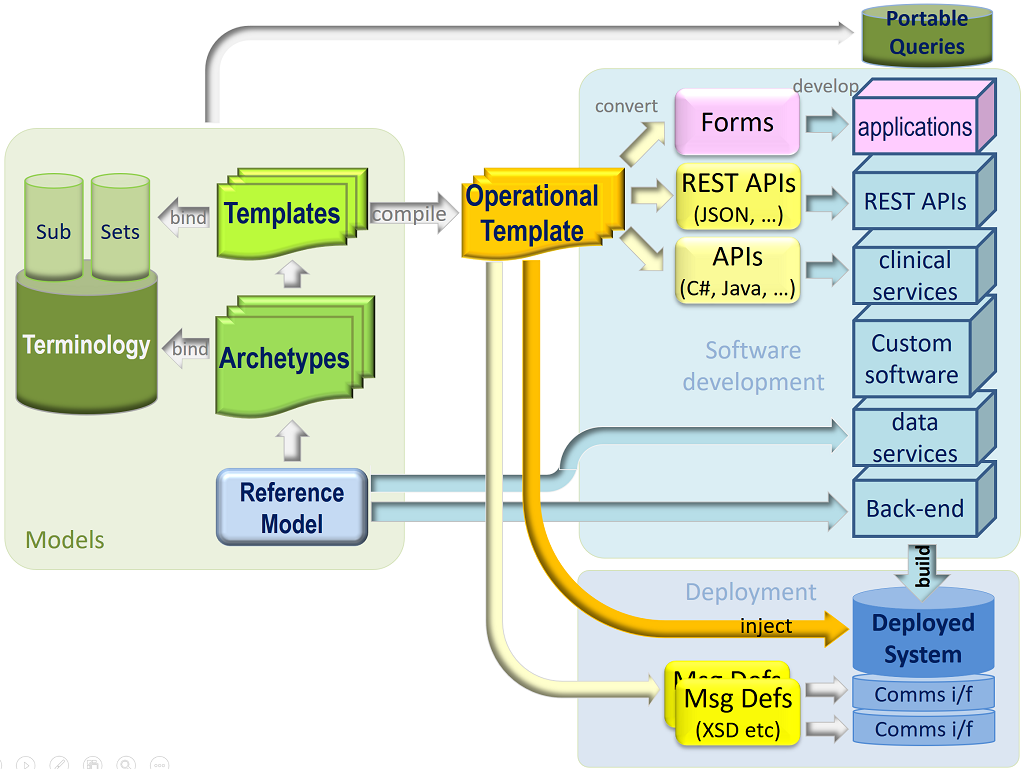
\includegraphics[scale=0.6]{./images/openehr_dev_ecosystem}
  \caption{Enfoque openEHR (Fuente: Extraído desde \cite{openEHR})}
  \label{fig:openeEHR_ecosystem}
\end{figure}
